 The given lines  can be written as
\begin{align}
\label{eq:chapters/12/11/2/15/lines}
\begin{split}
\vec{x} &= \myvec{-1\\-1\\-1} + \kappa_1\myvec{7\\-6\\1}\\
\vec{x} &= \myvec{3\\5\\7} + \kappa_2\myvec{1\\-2\\1} 
\end{split}
\end{align}
with
\begin{align}
\vec{A} = \myvec{-1\\-1\\-1},\, \vec{B} &= \myvec{3\\5\\7},\,
\vec{M} = \myvec{7&1\\-6&-2\\1&1}
\end{align}
%
Substituting the above in 
	    \eqref{eq:chapters/12/11/2/16/lsq/rank},
\begin{align}
\myvec{7&1&\vrule&4\\-6&-2&\vrule&6\\1&1&\vrule&8}
\xleftrightarrow[R_3 \leftarrow R_3 - \frac{1}{7}R_1]{R_2 \leftarrow R_2 + \frac{6}{7}R_1}\\
	\myvec{7&1&\vrule&4\\[1ex]0&-\frac{8}{7}&\vrule&\frac{66}{7}\\[1ex]0&\frac{6}{7}&\vrule&-\frac{52}{7}}
\xleftrightarrow{R_3 \leftarrow R_3 + \frac{3}{4}R_2}\\
\myvec{2&3&\vrule&1\\[1ex]0&-\frac{7}{2}&\vrule&\frac{1}{2}\\[1ex]0&0&\vrule&-\frac{5}{14}}
\end{align}
The rank of the matrix is 3. So the given lines are skew.
        From \eqref{eq:chapters/12/11/2/16/lsq/vec-eqn}
\begin{align}
\myvec{7&-6&1\\1&-2&1} \myvec{7&1\\-6&-2\\1&1}\bm{\kappa} &= \myvec{7&-6&1\\1&-2&1} \myvec{4\\6\\8}\\
\implies \myvec{86&20\\20&6}\bm{\kappa} &= \myvec{0\\0}
\label{eq:chapters/12/11/2/15/3}
\\
\implies \myvec{\kappa_1\\-\kappa_2} &= \myvec{0\\0}
\end{align}
From \eqref{eq:chapters/12/11/2/15/lines}, 
the closest points are $\vec{A}$  and $\vec{B}$ and  
the minimum distance between the lines is given by
\begin{align}
\norm{\vec{B}-\vec{A}} &= \norm{\myvec{4\\6\\8}}
= 2\sqrt{29}
\end{align}
%
See \figref{fig:chapters/12/11/2/15/}.
\begin{figure}[H]
\centering
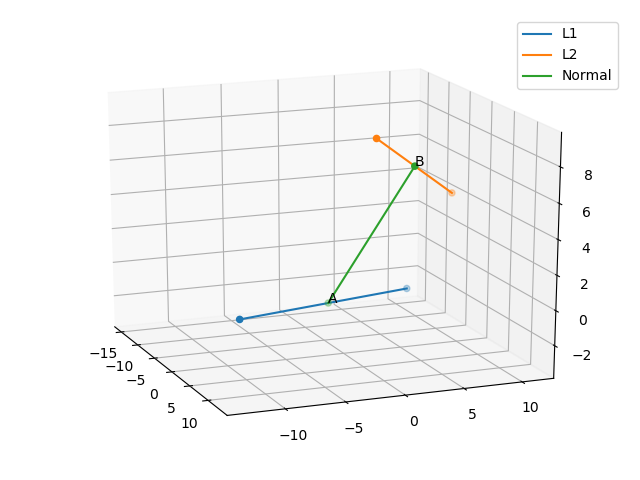
\includegraphics[width=0.75\columnwidth]{chapters/12/11/2/15/figs/Figure_1.png}
\caption{}
\label{fig:chapters/12/11/2/15/}
\end{figure}

